        \clearpage
        \begin{figure*}[ht]
            \pdfbookmark[2]{ID 05}{figure_id_05}
        	\centering
            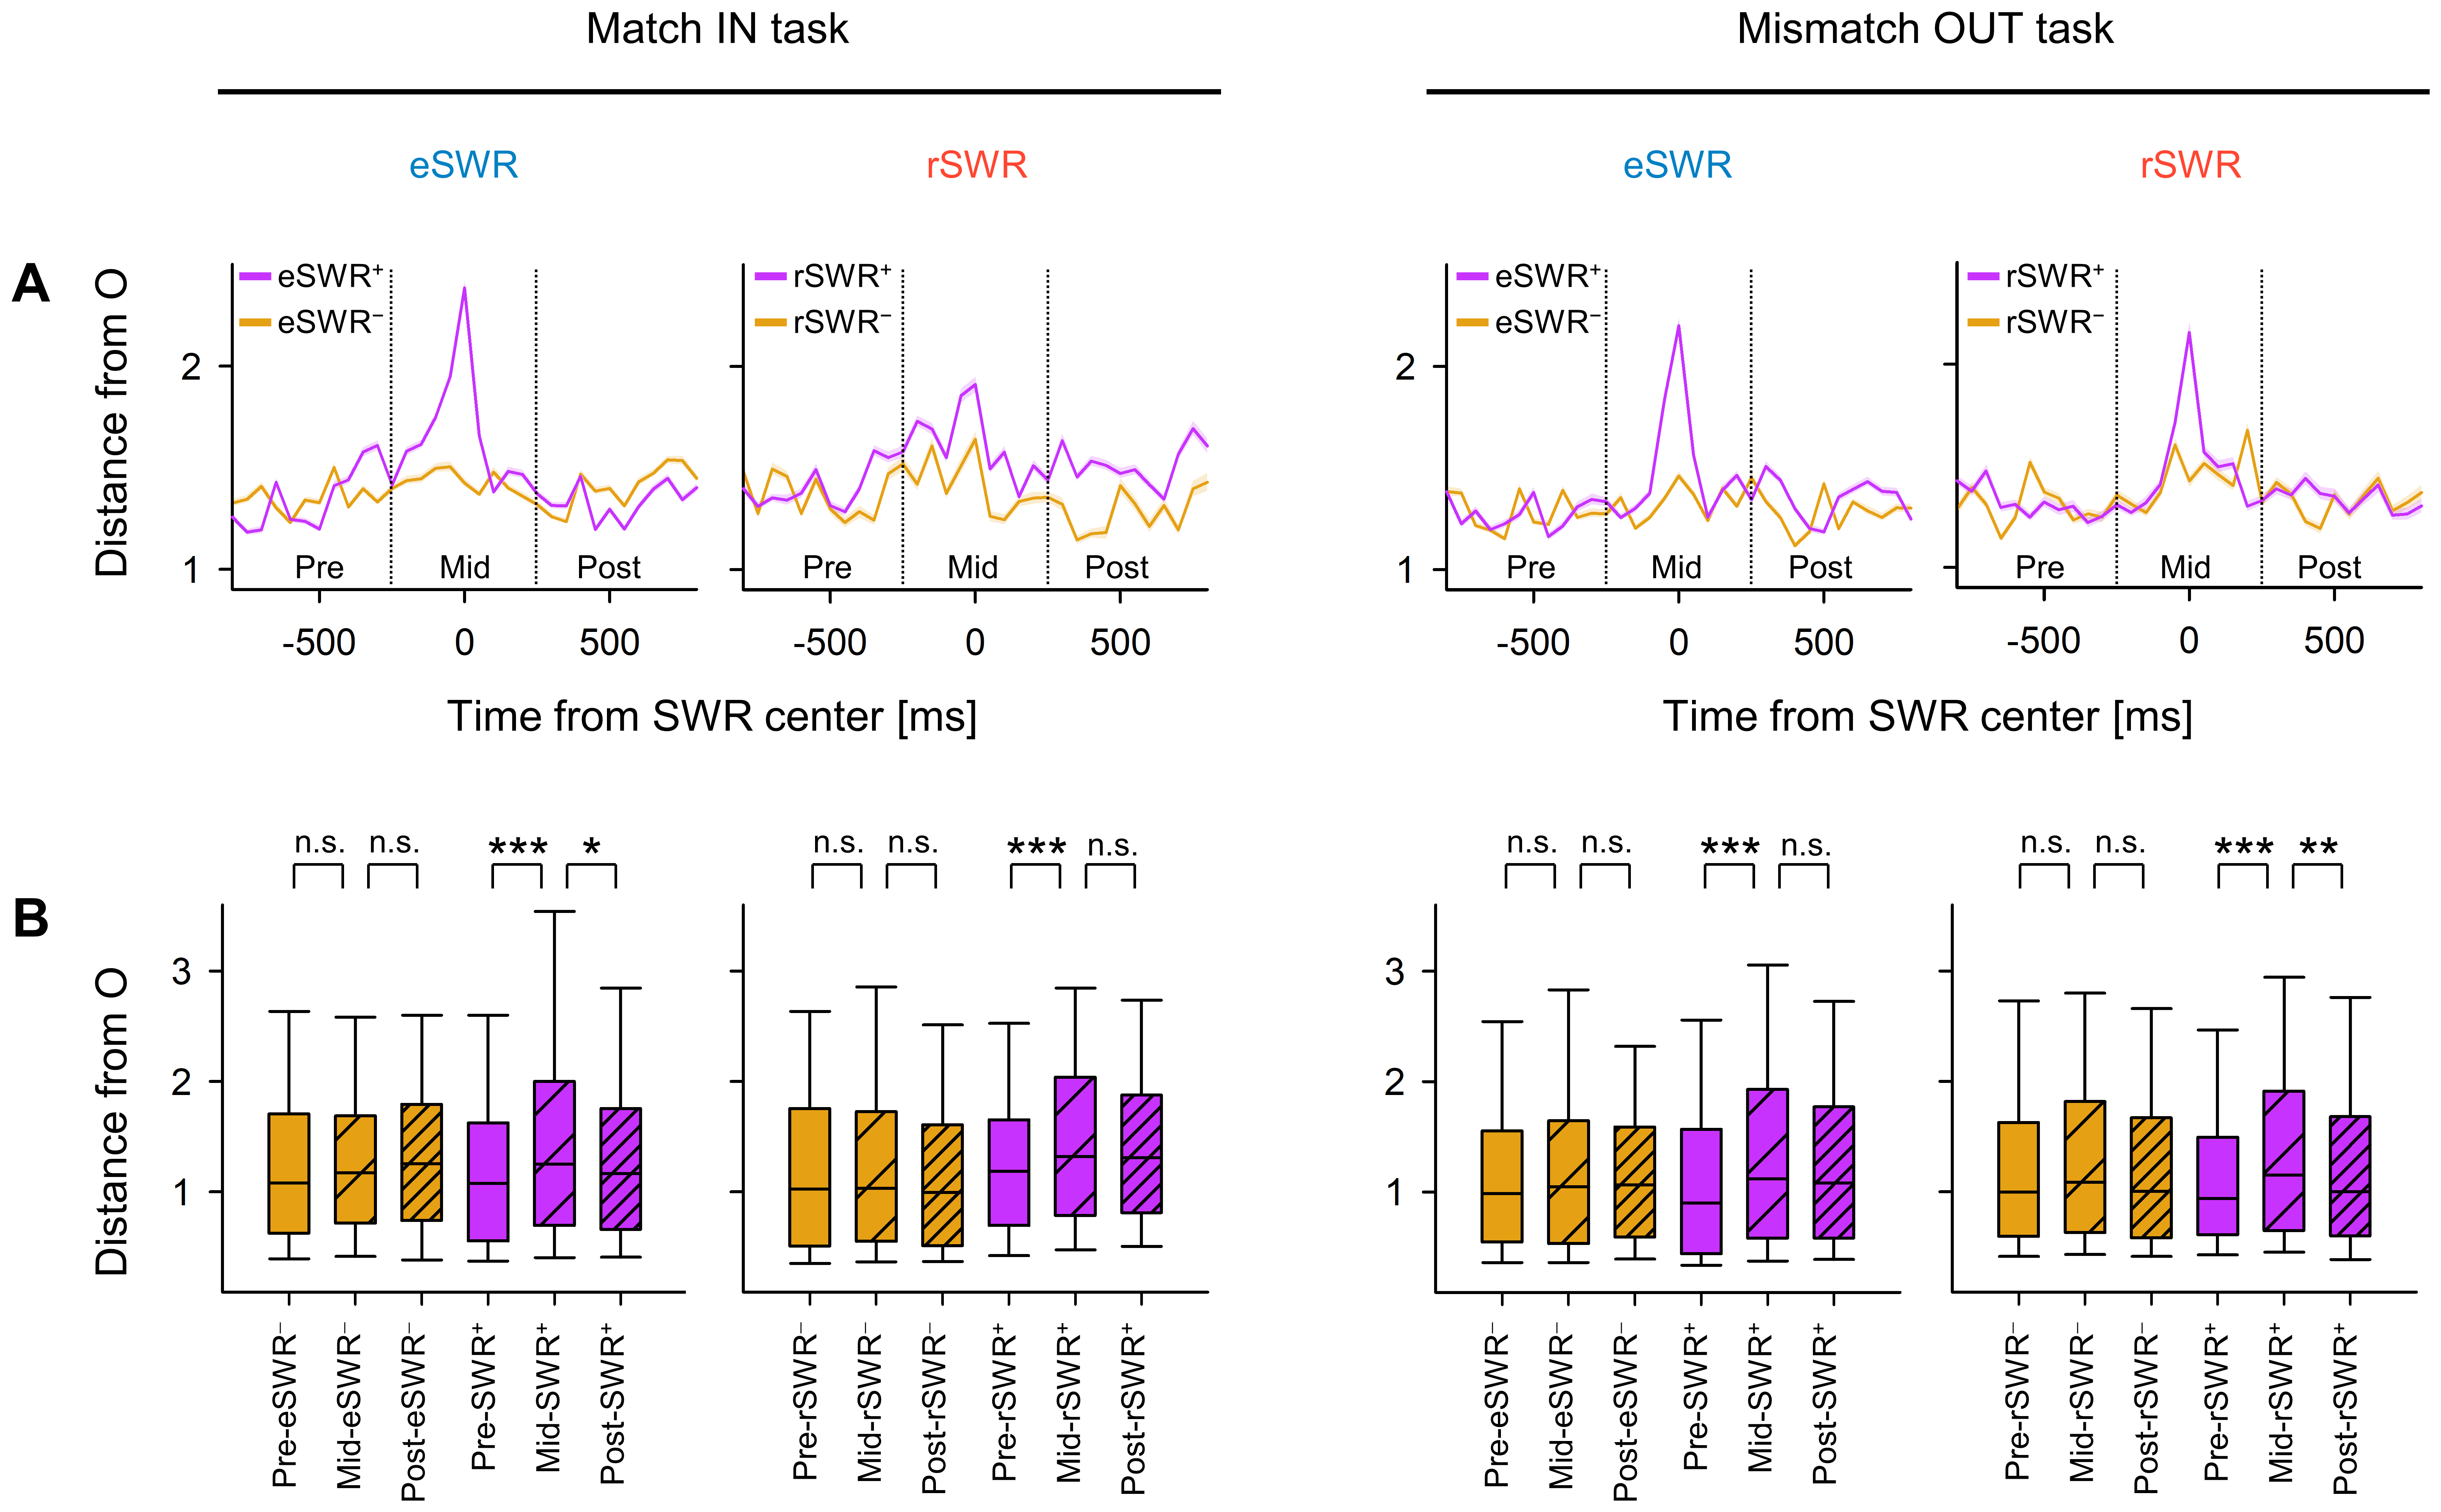
\includegraphics[width=1\textwidth]{./src/figures/.png/Figure_ID_05.png}
        	\caption{\textbf{Transient Change in Neural Trajectory during Sharp-Wave Ripple Events}
\smallskip
\\
\textbf{\textit{A.}} Distance from origin ($O$) of the peri-sharp-wave-ripple neural trajectory (mean \textpm 95\% confidence interval). Intervals may be inconspicuous due to their minimal ranges. \textbf{\textit{B.}} Distance from the origin ($O$) during the pre-, mid-, and post-sharp-wave ripple periods is demonstrated (*\textit{p} $<$ 0.05, **\textit{p} $<$ 0.01, ***\textit{p} $<$ 0.001; Brunner--Munzel test applied). Abbreviations: SWR, sharp-wave ripple event; eSWR, sharp-wave ripple during the encoding phase; rSWR, sharp-wave ripple within the retrieval phase; SWR$^+$, positive sharp-wave ripple event; SWR$^-$, control events for SWR$^+$; pre-, mid-, or post-SWR refer to the time intervals from $-800$ to $-250$ ms, from $-250$ to $+250$ ms, or from $+250$ to $+800$ ms, respectively, all relative to the center of the sharp-wave ripple event.}
% width=1\textwidth
        	\label{fig:05}
        \end{figure*}
